\chapter{Adquisición y limpieza de los datos}\label{chap:adq}

En cualquier proyecto de Data Science es necesario trabajar con una cantidad relativamente grande de datos. Sin embargo, normalmente el estado y el formato en el que se encuentran los datos de los que puede disponerse en Internet no se adecúan a las necesidades concretas del proyecto. Además, es habitual encontrar fuentes de datos con un número elevado de campos; es también tarea de esta etapa obtener los campos necesarios para el proyecto con el fin de aligerar las ejecuciones, ya que la mayoría de modelos son sensibles a la cantidad de campos. Por tanto, el proceso de adquisición y limpieza de los datos se convierte en una parte muy importante del proceso. Los objetivos principales de la etapa de limpieza de los datos son los siguientes:
\begin{itemize}
    \item Adaptar el formato a los requerimientos del proyecto.
    \item Eliminar registros incorrectos.
    \item Completar registros en los que falte alguno de los datos.
    \item Dejar únicamente los campos necesarios para el proyecto a desarrollar.
\end{itemize}

Para la creación del sistema de recomendación de películas basado en contenido que se desarrollará en este proyecto se utilizará un dataset consistente en información sobre varios miles de películas disponible en \url{https://github.com/harshitcodes/tmdb_mo}. El dataset consiste en dos ficheros: películas y créditos. Los campos disponibles en los ficheros son los siguientes:

\begin{itemize}
    \item Películas
    \begin{itemize}
        \item budget: Presupuesto de la película en Dólares.
        \item genres: Generos cinematográficos asociados a la película.
        \item homepage: Página web de la productora de la película.
        \item id: Identificador único dentro del dataset.
        \item plot\_keywords: Palabras clave.
        \item original\_language: Idioma original
        \item original\_title: Título original de la película
        \item overview: Resumen
        \item popularity: Popularidad (unidades desconocidas)
        \item production\_companies: Compañías encargadas de la producción
        \item production\_countries: Paises productores de la película
        \item release\_date: Fecha de lanzamientoç
        \item revenue: Recaudación
        \item runtime: Días en cartelera
        \item spoken\_languages: Idiomas hablados
        \item status: Estado de la película
        \item tagline: Subtítulo
        \item title: Título en inglés
        \item vote\_average: Promedio de votos
        \item vote\_count: Número de votos
    \end{itemize}
    \item Créditos
    \begin{itemize}
        \item movie\_id: Identificador de la película (para unirlo con el dataset anterior).
        \item title: Título en inglés de la película
        \item cast: Actores que aparecen (en orden e importancia)
        \item crew: Equipo participante en la película
    \end{itemize}
\end{itemize}

\section{Importación de datos}

El primer paso en la etapa de adquisición de los datos consiste en leer ambos ficheros (en formato csv) y obtener los DataFrame de Pandas correspondintes. Las columnas genres, keywords, production\_countries, production\_companies, spoken\_languages, cast y crew están en formato json en origen. Es por ello que en las funciónes de lectura de los datos tienen un trato especial. Las funciones implementadas son las siguientes:

\begin{lstlisting}[language=Python, caption=Lectura de los datos del fichero de películas.]
import json
import pandas as pd
def load_tmdb_movies(path):
    """Función utilizada para cargar el dataset de las películas. Se transforma a fecha el campo de fecha de salida
    y se cargan como listas los campos que están guardados como json.
    Args:
        path (str): Ruta hasta el archivo de tmdb_5000_movies.csv
    Returns:
        pd.DataFrame: Dataframe de pandas con la información del csv
    """
    df = pd.read_csv(path)
    df['release_date'] = pd.to_datetime(df['release_date']).apply(lambda x: x.date())
    json_columns = ['genres', 'keywords', 'production_countries', 'production_companies', 'spoken_languages']
    for column in json_columns:
        df[column] = df[column].apply(json.loads)
    return df
\end{lstlisting}

\begin{lstlisting}[language=Python, caption=Lectura de los datos del fichero de créditos.]
def load_tmdb_credits(path):
    """Función utilizada para cargar el dataset de los créditos. Se cargan como listas los campos que están guardado
    Args:
        path (str): Ruta hasta el archivo de tmdb_5000_credits.csv
    Returns:
        pd.DataFrame: [description]
    """
    df = pd.read_csv(path)
    json_columns = ['cast', 'crew']
    for column in json_columns:
        df[column] = df[column].apply(json.loads)
    return df
\end{lstlisting}

Pandas es una librería rápida, flexible, opensource y relativamente fácil de usar. Está implementada en Python y es una de las librerías más usadas para realizar tareas de análisis y manipulación de datos. En este proyecto esta librería será utilizada de forma extensiva. Con estas dos funciones se consigue tener los datos en el tipo de dato que proporciona Pandas, el DataFrame. Este tipo de objeto tiene formato tabular (donde una fila es un registro y una columna un atributo del registro) y tiene multitud de métodos implementados para la transformación de datos.\\

En esta primera etapa de importación, el objetivo es obtener un único DataFrame que contenga información de ambos conjuntos de datos. Un problema habitual que tiene lugar al juntar dos ficheros es la información faltante de los ficheros. Hay que tratar de forma especial el acceso a los datos de cada DataFrame a la hora de juntarlos, pues puede que haya campos que no estén informados. Para ello, definimos una función que accede de forma segura a los datos, ya que en caso de no encontrarlo devuelve nulo, evitando errores de ejecución.

\begin{lstlisting}[language=Python, caption=Acceso a los datos de forma segura.]
def safe_access(container, index_values):
    """Función para acceder de forma segura a valores. En caso de que no se encuentre uno de ellos, se devuelve NaN
    en vez de lanzar un error.
    Args:
        container (list): Lista/ contenedor de la que quieren extraerse los valores
        index_values (list): Lista de índices a extraer del contenedor
    Returns:
        any: Valores extraidos
    """
    result = container
    try:
        for idx in index_values:
            result = result[idx]
        return result
    except IndexError or KeyError:
        return pd.np.nan
\end{lstlisting}

Uno de los campos a extraer del fichero de créditos es el de director. Este campo se encuentra dentro del campo de crew (en formato json) con la clave director. Por tanto, para añadirlo al DataFrame es necesario buscarlo. Para ello se define la función get\_director.
\begin{lstlisting}[language=Python, caption= Obtención de una lista de directores extraidos del campo crew.]
def get_director(crew_data):
    """Devuelve el director dado un json con toda la composición del equipo de la película.
    Args:
        crew_data (json): JSON con el equipo que ha realizado la película
    Returns:
        str: Director de la película
    """
    directors = [x['name'] for x in crew_data if x['job'] == 'Director']
    return safe_access(directors, [0])
\end{lstlisting}

Como se ha visto anteriormente, el objetivo del proyecto es crear un sistema de recomendación de películas basado en contenido. Por tanto, resulta vital conseguir información del contenido de las películas. El campo fundamental para conseguir este fin es el campo keywords, que contiene las palabras clave de cada película. Este campo está en origen en formato json, con información que no es relevante para el objetivo del proyecto. Para obtener únicamente las palabras clave se implementa pipe\_flatten\_names que extrae estas palabras clave.
\begin{lstlisting}[language=Python, caption= Extracción de las palabras clave a partir del JSON del DataFrame.]
def get_director(crew_data):
    """Devuelve el director dado un JSON con toda la composición del equipo de la película.
    Args:
        crew_data (json): JSON con el equipo que ha realizado la película
    Returns:
        str: Director de la película
    """
    directors = [x['name'] for x in crew_data if x['job'] == 'Director']
    return safe_access(directors, [0])
\end{lstlisting}

Para terminar con la etapa de importación y carga de los datos, se crea la función que añade al DataFrame de películas la información de credits necesaria.
\begin{lstlisting}[language=Python, caption=]
def convert_to_original_format(movies, credits):
    """Aplica una serie de funciones para añadir información al dataset de películas a partir del
    conjunto de datos de créditos
    Args:
        movies (pd.DataFrame): DataFrame obtenido de leer el archivo de películas
        credits (pd.DataFrame): DataFrame obtenido de leet el archivo de créditos
    Returns:
        pd.DataFrame: DataFrame con la información conjunta
    """
    tmdb_movies = movies.copy()
    tmdb_movies.rename(columns=TMDB_TO_IMDB_SIMPLE_EQUIVALENCIES, inplace=True)
    tmdb_movies['title_year'] = pd.to_datetime(tmdb_movies['release_date']).apply(lambda x: x.year)
    # I'm assuming that the first production country is equivalent, but have not been able to validate this
    tmdb_movies['country'] = tmdb_movies['production_countries'].apply(lambda x: safe_access(x, [0, 'name']))
    tmdb_movies['language'] = tmdb_movies['spoken_languages'].apply(lambda x: safe_access(x, [0, 'name']))
    tmdb_movies['director_name'] = credits['crew'].apply(get_director)
    tmdb_movies['actor_1_name'] = credits['cast'].apply(lambda x: safe_access(x, [1, 'name']))
    tmdb_movies['actor_2_name'] = credits['cast'].apply(lambda x: safe_access(x, [2, 'name']))
    tmdb_movies['actor_3_name'] = credits['cast'].apply(lambda x: safe_access(x, [3, 'name']))
    tmdb_movies['genres'] = tmdb_movies['genres'].apply(pipe_flatten_names)
    tmdb_movies['plot_keywords'] = tmdb_movies['plot_keywords'].apply(pipe_flatten_names)
    return tmdb_movies
\end{lstlisting}

Por último, se cargan las librerías necesarias para el proyecto y se leen los datos de los ficheros, usando las funciones definidas anteriormente.
\begin{lstlisting}[language=Python, caption=Código usado para la carga de los datos.]
import pandas as pd
import numpy as np
import matplotlib as mpl
import matplotlib.pyplot as plt
import seaborn as sns
import math, nltk, warnings
from nltk.corpus import wordnet
from sklearn import linear_model
from sklearn.neighbors import NearestNeighbors
from fuzzywuzzy import fuzz
from wordcloud import WordCloud, STOPWORDS
plt.rcParams["patch.force_edgecolor"] = True
plt.style.use('fivethirtyeight')
mpl.rc('patch', edgecolor = 'dimgray', linewidth=1)
from IPython.core.interactiveshell import InteractiveShell
InteractiveShell.ast_node_interactivity = "last_expr"
pd.options.display.max_columns = 50
%matplotlib inline
warnings.filterwarnings('ignore')

#Definimos la función a utilizar para obtener el lexema de las palabras.
PS = nltk.stem.PorterStemmer()
# load the dataset
credits = load_tmdb_credits("./datos/tmdb_5000_credits.csv")
movies = load_tmdb_movies("./datos/tmdb_5000_movies.csv")
df_initial = convert_to_original_format(movies, credits)
\end{lstlisting}

Con esto, se consigue tener un único DataFrame sobre el que trabajar.

\section{Limpieza y transformación de los datos}

Una vez se han importado y cargado los datos, la siguiente etapa es el limpiado de los datos, tanto para lidiar con los posibles datos faltantes.

\subsection{Entradas duplicadas}

En ocasiones los DataSets que se encuentran en Internet no están en un estado perfecto, y en ocasiones se tienen datos duplicados. Es importante comprobar si existen datos duplicados, ya que si no a la hora de crear modelos puede darse más importancia a unos registros que a otros, lo cual resulta un error de concepto. En primer lugar, por tanto, comprobamos la existencia de entradas duplicadas.
\begin{lstlisting}[language=Python, caption=Entradas duplicadas]
doubled_entries = df_initial[df_initial.id.duplicated()]
doubled_entries.shape
\end{lstlisting}
El resultado es que no existen entradas duplicadas. Sin embargo, comprobar la duplicidad de esta forma tan genérica puede no solucionar todos los posibles problemas. Por ejemplo, podría haber una entrada con un error ortográfico o con diferencias mínimas. En este caso, cada entrada se corresponde con una película, por lo que tener dos entradas que únicamente difieren en, por ejemplo, el presupuesto, podría considerarse una entrada duplicada. Dado que son datos de películas, buscaremos entradas con el mismo título. 

\begin{lstlisting}[language=Python, caption=Entradas con título duplicado.]
df_temp = df_initial
list_var_duplicates = ['movie_title', 'title_year', 'director_name']
liste_duplicates = df_temp['movie_title'].map(df_temp['movie_title'].value_counts() > 1)
df_temp[liste_duplicates][list_var_duplicates].sort_values('movie_title')
\end{lstlisting}

El resultado se muestra en la Tabla\ref{tab:duplicated_entries}. Como puede comprobarse, únicamente hay tres parejas de películas con el mismo título. Analizándolo a simple vista puede verse que se trata de remakes, por lo que no podemos considerarlo como entradas duplicadas, ya que pueden diferir en calidad e incluso en alguna palabra clave.
\begin{table}[h]
\centering
\begin{tabular}{llrl}
\toprule
\textbf{id} &     \textbf{movie\_title} &  \textbf{title\_year} &        \textbf{director\_name} \\
\midrule
1359 &           Batman &      1989 &           Tim Burton \\
4267 &           Batman &      1966 &  Leslie H. Martinson \\
3647 &  Out of the Blue &      1980 &        Dennis Hopper \\
3693 &  Out of the Blue &      2006 &       Robert Sarkies \\
972  &         The Host &      2013 &        Andrew Niccol \\
2877 &         The Host &      2006 &         Bong Joon-ho \\
\bottomrule
\end{tabular}
\caption{Entradas con el título duplicado.}
\label{tab:duplicated_entries}
\end{table}

Por tanto, puede concluirse que en el dataset no existen entradas duplicadas. A pesar de tener el mismo dataset al inicio de este apartado que ahora, se ha incluido por completitud, ya que es un paso que debe realizarse siempre.

\subsection{Limpieza de keywords}

Las keywords tendrán un papel fundamental en el funcionamiento del sistema. De hecho, como se verá en el Capítulo \ref{chap:creacion}, las recomendaciones se realizarán en base a la similaridad entre películas, y para esta medida se usarán las keywords. Por tanto, se hace necesario analizar el contenido de esta variable, puesto que se realizará un uso extensivo de ella.\\

Incialmente, el dataset contiene un total de 9474 keywords. En la Figura\ref{fig:keywords_histogram} se muestra la distribución del número de keywords. Puede verse que aun habiendo casi el doble de keywords que de películas, la mayoría de películas contienen entre 5 y 15 keywords, por lo que el número de keywords no es preocupante.
\begin{figure}[H]
    \centering
    \captionsetup{width=10cm}
    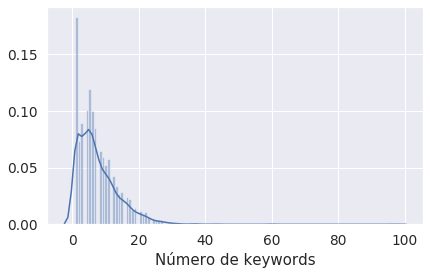
\includegraphics[width=12cm]{contenido/imagenes/keyword_histogram.png}
    \caption{Histograma con el número de keywords de cada película.}
    \label{fig:keywords_histogram}
\end{figure}

Sin embargo, tratar con lenguaje natural siempre implica poner especial atención en lo que se consideran palabras diferentes. Es lógico pensar que a la hora de poner las keywords de las películas no se ha tenido en cuenta las posibles similitudes entre keywords ni se han asignado de una lista cerrada.\\

Los seres humanos nos expresamos de forma muy diferente y probablemente las keywords hayan sido asignadas por personas diferentes. Por lo cual es esperable que haya keywords que signifiquen aproximadamente lo mismo pero que por tener distintas grafías actualmente se considerarían diferentes palabras.\\

El lenguaje de Python es ampliamente utilizado en la disciplina de la ciencia de datos, es por ello que existen numerosas liberías de inestimable ayuda para el NLP. Una de las más conocidas es NLTK (\textbf{N}atural \textbf{L}anguage \textbf{T}ool\textbf{K}it).